\documentclass{article}
\usepackage[a4paper, total={6in, 8in}]{geometry}
\usepackage{graphicx}
\usepackage{amsmath,amssymb}


\begin{document}

\begin{table*}
  \small
  \begin{centering}
    \begin{tabular}{l | l | c c | c c c | c}
      \hline
      \hline
        Object         &  MJD         &  \multicolumn{2}{c}{Cont. @ 1450\AA }                        &   \multicolumn{3}{c}{CIV 1549\AA}                                   & Virial product \\
                       &              &       $\nu L_{\nu}$    &         Slope                       &   Luminosity             &     FWHM           &    V$_{\rm off}$    & log($\nu L_{\nu}^{0.5} \times {\rm FWHM}^2$)\\
                       &              & $10^{42}$ erg s$^{-1}$ & (F$_\lambda \propto \lambda^\alpha$)  & $10^{42}$ erg s$^{-1}$ &     km s$^{-1}$    &    km s$^{-1}$      &  $\log(M)$ \\
      \hline                        
                       &  53498       &  38129   $\pm$ 39      &  -1.57 $\pm$ 0.01                   &  898    $\pm$ 15         &   6024 $\pm$  120  &     944 $\pm$  33   &   9.85 $\pm$ 0.02\\
          J1205+3422   &  58538       &   8550   $\pm$ 11      &  -1.41 $\pm$ 0.01                   &  385.2  $\pm$  3.9       &   7109 $\pm$   91  &    1085 $\pm$  29   &   9.67 $\pm$ 0.01\\  
                       &  58693$^*$   &   2725   $\pm$ 40      &  -1.27 $\pm$ 0.05                   &  161    $\pm$ 22         &  14997 $\pm$ 2500  &     922 $\pm$ 690   &  10.07 $\pm$ 0.13\\  
                                      &                        &                                     &                          &                    &                     &                  \\
                       &  54553       &   3579   $\pm$ 49      &  -1.16 $\pm$ 0.07                   &  293.6  $\pm$  8.8       &   4630 $\pm$  180  &     183 $\pm$  57   &   9.11 $\pm$ 0.04\\  
          J1638+2827   &  55832       &   2340   $\pm$ 15      &  -2.17 $\pm$ 0.05                   &   84.6  $\pm$  4.2       &   4733 $\pm$  290  &     172 $\pm$  89   &   9.04 $\pm$ 0.05\\  
                       &  58583       &   7793   $\pm$ 19      &  -2.02 $\pm$ 0.01                   &  367.5  $\pm$  4.3       &   4511 $\pm$   71  &      94 $\pm$  24   &   9.25 $\pm$ 0.01\\  
                                      &                        &                                     &                          &                    &                     &                  \\
                       &  56189$^*$   &    607   $\pm$ 49      &  -0.00 $\pm$ 0.16                   &   72.8  $\pm$ 11.3       &  14993 $\pm$ 2400  &     828 $\pm$ 691   &   9.74 $\pm$ 0.14\\  
          J2228+2201   &  56960       &   7842   $\pm$ 25      &  -1.72 $\pm$ 0.02                   &  301.0  $\pm$  7.2       &   7136 $\pm$  210  &    -276 $\pm$  64   &   9.65 $\pm$ 0.03\\ 
                       &  58693       &   2388.4 $\pm$  6.8    &  -1.22 $\pm$ 0.01                   &  145.4  $\pm$  1.5       &   6084 $\pm$   83  &     168 $\pm$  28   &   9.26 $\pm$ 0.01\\  
      \hline
      \hline
    \end{tabular}
    \caption{Continuum (at 1450\AA) and CIV spectral measurements for the three QSO considered in this work, at all observation epochs, as calculated by QSFit.  The last column shows the virial product calculated as $\nu L_{\nu}^{0.5} \times {\rm FWHM}^2$.  $^*$: The CIV line is very faint (with respect to the continuum), and the associated estimates are likely biased.}
    \label{tab:QSFit-results}
  \end{centering}
\end{table*}

We analyzed the spectra of the three QSO considered in this work, at all observation epochs, using the QSFit spectral fitting package \citep{Calderone2017}.  In this case the main advantage of using QSFit is that it allows to constrain the slope and luminosity of the broad band continuum of the source, using data at all available wavelengths. The relevant estimated quantities are shown in Tab.~\ref{tab:QSFit-results}, and the plot of the best fit model in the region of the CIV emission line are shon in Fig.~\ref{fig:QSFit-CIV}.  We used the standard settings in all analysis, except for the CIV emission line profile for which we used a Lorentzian profile (rather than a Gaussian one).  The latter allows to account for the rather narrow peak of the CIV line without adding a further, and typically highly degenerate, ``narrow'' line component to the model.  Only in two cases where the CIV line became barely distinguishable (marked with a $^*$ in Tab.~\ref{tab:QSFit-results}) a narrow component appeared in the spectra.  The latter is however much fainter than the main broad components detected at other epochs, hence we neglect it.

The QSO continuum (here evaluated at 1450\AA) and the CIV line luminosities follow a similar evolution, with a ratio of $\sim$~20--30, confirming that the main driver for emission line variability is likely the broad band continuum itself.  Also, for all sources except J1638+2827, the slope of the continuum changes with luminosity following a bluer-when-brighter pattern, suggesting that a distinct emerging component is responsible or both the slope and luminosity variations.  In J1638+2827 the opposite beahviour is observed, especially in the first observation epoch.  However, this may be a bias due to the limited wavelength range available which extends to $\lambda \sim 1240\AA$ for the first epoch, while it extend to shorter wavelengths for the other epochs (respectively 1140\AA and 1010\AA).  The latter suggests that the ``emerging'' component is more prominent at UV wavelengths, and a sufficent wavelength coverage is required to detect it.

In all cases where the CIV line profile is reliably constrained its FWHM is rather constant, with maximum variations $\lesssim$~1000 km s$^{-1}$, despite the significantly larger variations in the line luminosities.  The FWHM of broad lines is likely related to the mass of the supermassive black hole powering the QSO phenomenon, which is supposed to be constant on any human timescale.  Hence it is instructive to check whether the virial product, which is the basic quantity used to calculate the single epoch mass estimate, show any variation.  The virial product, calculated as $\nu L_{\nu}^{0.5} \times {\rm FWHM}^2$, is reported in the last column of Tab.~\ref{tab:QSFit-results}.  The uncertainty typically associated to the single epoch mass estimate is $\sim$~0.5 dex, hence the virial product at all epochs are remarkably constant and compatible with a single value of black hole mass for each source, even in those cases where the CIV estimates are possibly unreliable.  The object showing larger variation is J2228+2201, although the extreme values span a range of 0.48 dex.

Finally, also the velocity offsets of the CIV line are rather constant, and compatible with a single value (within 3$\sigma$).  The only exception is J2228+2201, where a significant change ($\sim 7 \sigma$) is observed between the second and third observation epochs.


\begin{figure*}
  \centering
  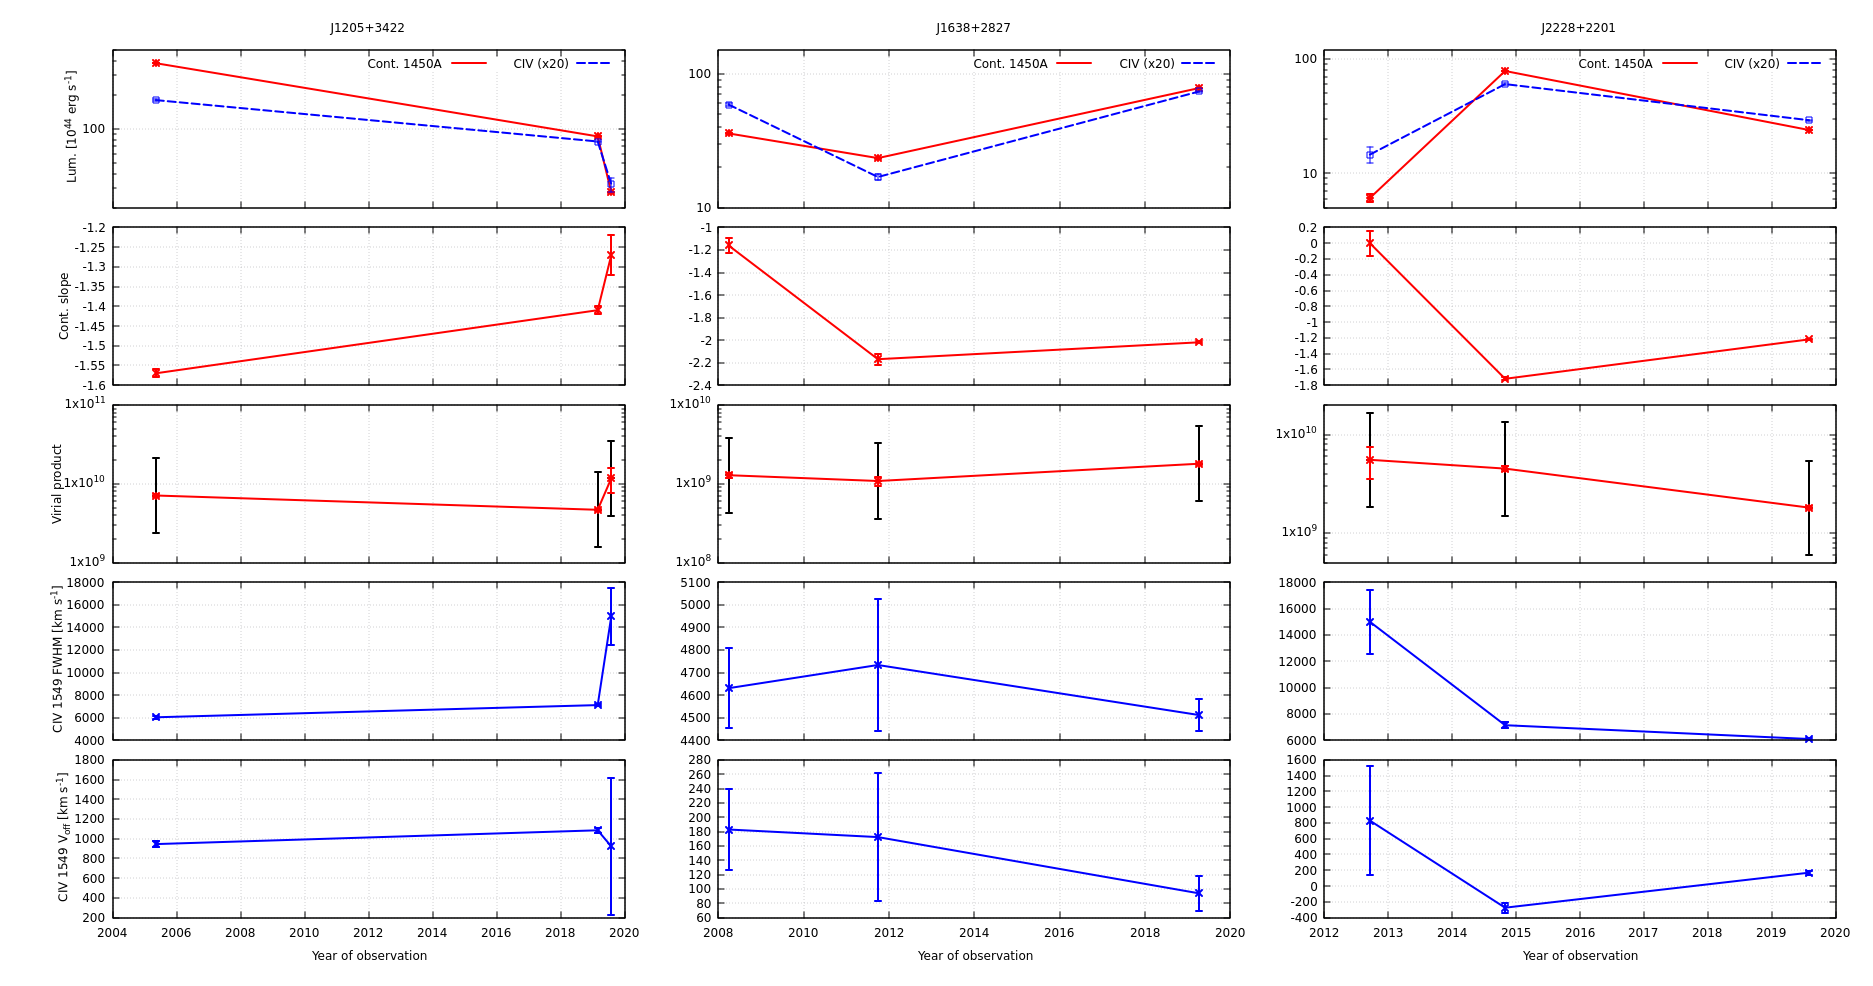
\includegraphics[width=\textwidth]{QSFit-results}
   \vspace{-12pt}
   \caption{Temporal evolution of the Spectral properties of the three QSO considered in this work (Tab.~\ref{tab:QSFit-results})}.
     \label{fig:QSFit-results}
\end{figure*}



\begin{figure*}
  \centering
  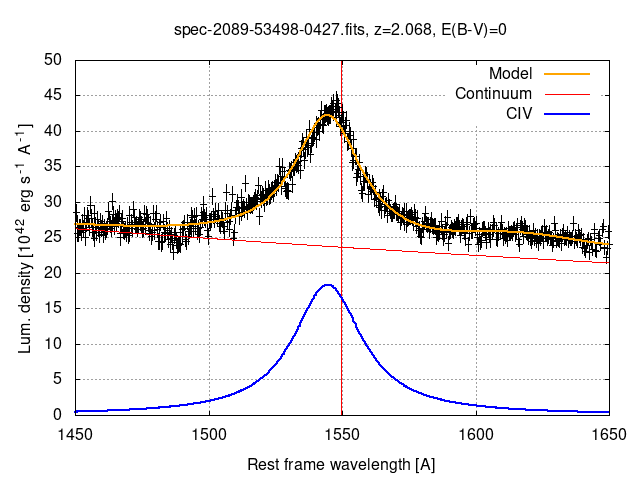
\includegraphics[width=.3\textwidth]{spec-2089-53498-0427}
  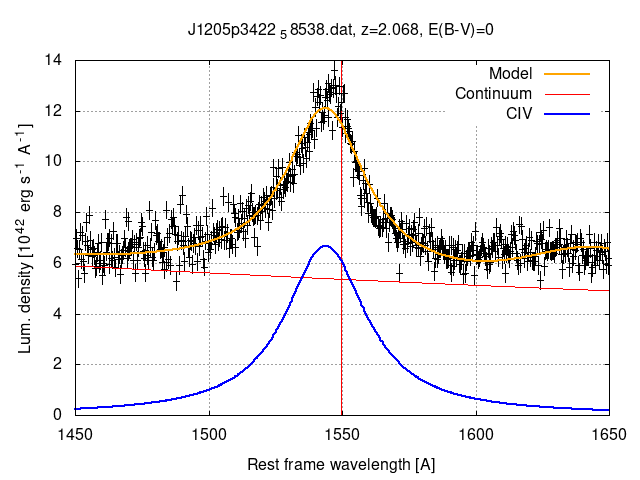
\includegraphics[width=.3\textwidth]{J1205p3422_58538}
  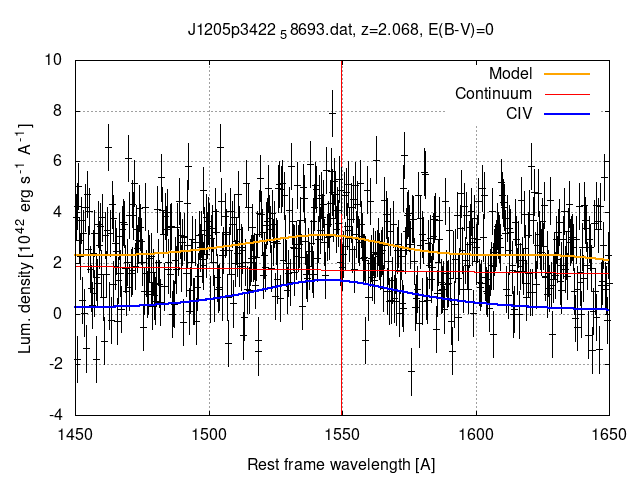
\includegraphics[width=.3\textwidth]{J1205p3422_58693}\\
  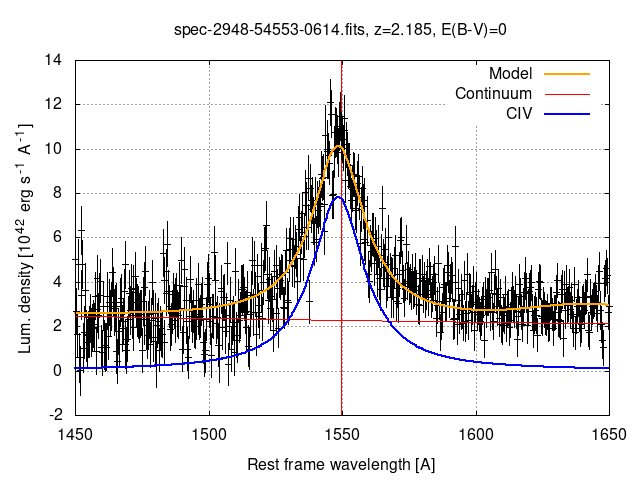
\includegraphics[width=.3\textwidth]{spec-2948-54553-0614}
  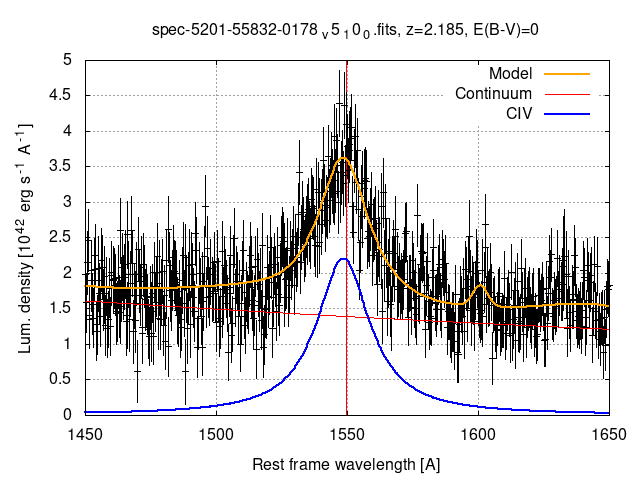
\includegraphics[width=.3\textwidth]{spec-5201-55832-0178_v5_10_0}
  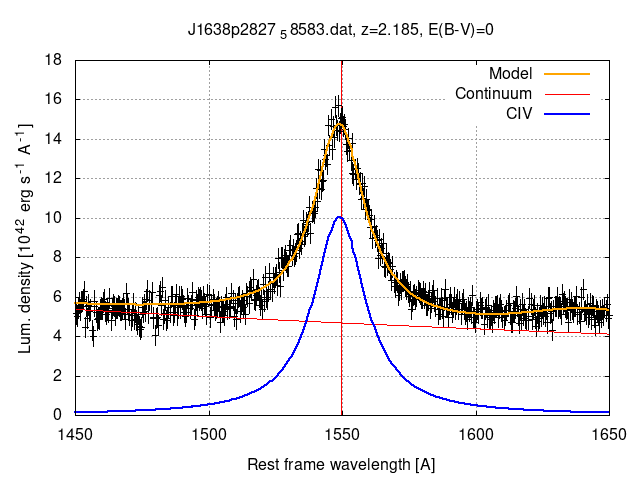
\includegraphics[width=.3\textwidth]{J1638p2827_58583}\\
  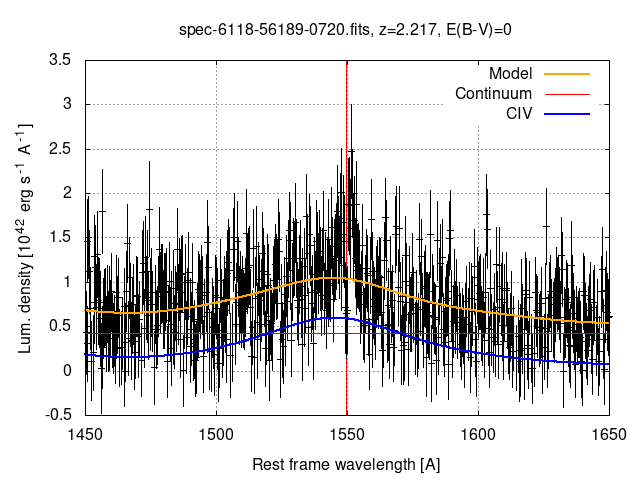
\includegraphics[width=.3\textwidth]{spec-6118-56189-0720}
  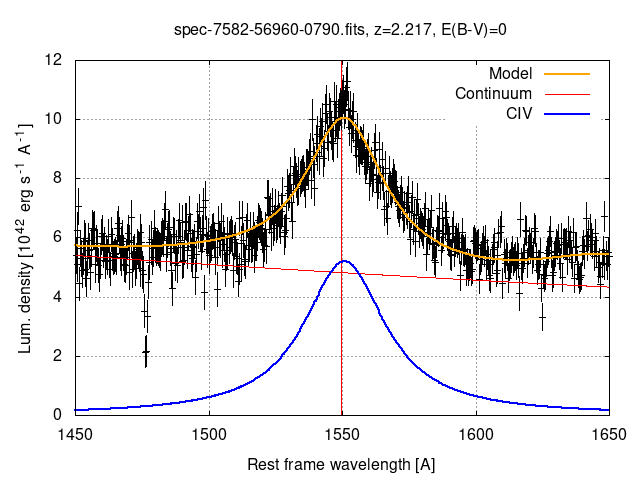
\includegraphics[width=.3\textwidth]{spec-7582-56960-0790}
  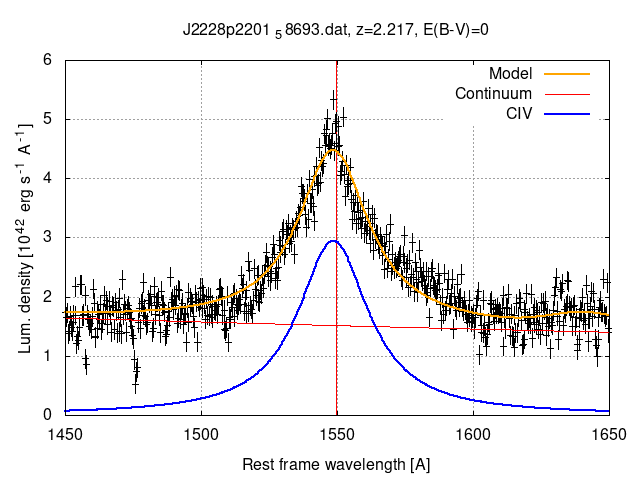
\includegraphics[width=.3\textwidth]{J2228p2201_58693}
  \caption{Observed spectra and best fit model in the region relevant to CIV emission line for all QSO considered in this work}.
  \label{fig:QSFit-CIV}
\end{figure*}
\end{document}

\end{document}
